\chapter{Environment}
This section will explain how to set up and start a bot with the StarCraft environment using the GOAL programming language.

\section{Installation}
For full installation instructions, see: \url{https://github.com/eishub/StarCraft/wiki/Install-Guide}

\section{Chaoslauncher}
In order to make use of all the StarCraft Brood War plugins, you can make use of the Chaoslauncher application. With this application, several plugins can be used like the \textit{BWAPI Injector} which is necessary for using the BWAPI library. It is also recommended to make use of the \textit{APMAlert} plugin, which shows the current actions per minute of all your units together. When the APM of your bot is suddenly very high, your agents might be executing too many actions in a row. It is also recommended to make use of the \textit{W-Mode} plugin. This plugin automatically starts your StarCraft game in windowed mode which is easier for debugging. Yu can also make use of the \textit{ChaosPlugin} to make use of its autoreplay function which automatically saves a replay at the end of each game. You can play these replays by first turning off the \textit{BWAPI Injector}. You can then start StarCraft (in the launcher) and select \textit{Single Player} with gametype \textit{Expansion}. Press the `Ok' button and then the `Load Replay' button. If you then open the 
\texttt{Autoreplay} directory in that screen you should be able to see all the replays which are saved by the autoreplay function.

\section{The Mas2g}
\label{mas2g}
The StarCraft environment offers multiple parameters to be set up in the mas2g. Within the mas2g you can specify which map you want to play, specify your own race, set the location of your StarCraft game, turn the development tool on or off, enable the automenu script, and specify which race you want to play against. When any of these parameters are updated, do not forget to close the Chaoslauncher before launching the mas2g, or else your changes will not be applied.

\begin{verbatim}
    use "../../StarCraft Connector.jar" as environment with
        map="(2)Destination.scx",
        own_race="terran",
        StarCraft_location="C:\\StarCraft",
        debug="true",
        auto_menu="Single_Player",
        enemy_race="zerg",
        game_speed=50.
\end{verbatim}

\subsection{Map}
\label{map}
It is possible to specify which map the Chaoslauncher will automatically load when starting the game. This can be done by inserting the following line: \textit{map = <filename>}, where \textit{<filename>} is the exact filename of the map (with extension). Please note that the environment only supports maps in the directory: \textit{StarCraft/maps/sscai}. Please note that the first time running the environment on a certain map will take some time (around 2 minutes) to generate the API data of the given map.

\subsection{Own Race}
\label{own race}
You may also specify the race of your bot in the mas2g. This will automatically launch the Chaoslauncher with the specified race. You can do this by inserting the following line: \textit{own\_race = <RaceName>}, where \textit{<RaceName>} can either be \textit{zerg}, \textit{protoss}, \textit{terran} or \textit{random}. The option \textit{random} will choose one race with a 1/3 chance for each race.

\subsection{StarCraft Location}
\label{StarCraft location}
It is also possible to specify the location of the StarCraft game. When using the StarCraft game provided by the environment installer, this feature will automatically start the Chaoslauncher when launching the GOAL MAS. When the Chaoslauncher is already running, it will not start again until you close it, but this is fine as long as you use the same init parameters. When the Choaslauncher is automatically started by the environment, an automatic script will be written with all the necessary information to run the GOAL agents (so it is recommended to use this feature). You can use this feature by inserting the line: \textit{StarCraft\_location = <FilePath>}, where \textit{<FilePath>} is the absolute path to the StarCraft installation folder.

\subsection{Debug}
\label{debug}
The environment also offers a development tool for debugging purposes. With this development tool, you can increase or decrease the game speed, enable cheats and draw unit and map details on the screen. More information about the development tool can be found at \ref{development tool}. In order to enable or disable launching the development tool, you can insert the following line: \textit{debug=<Boolean>}.

\subsection{Auto Menu}
\label{auto menu}
The auto menu parameter can be used to automatically go through the menus of the game when starting your agents. This can be used for single player games and multi player games. To use the auto menu function you can insert the following line: \textit{auto\_menu=<MenuChoice>}, where \textit{<MenuChoice>} is either \textit{Single\_Player} for a single player game or \textit{Multi\_Player} for a multi player game.

\subsection{Enemy Race}
\label{enemy race}
The enemy race parameter can be used for specifying which race you want to play against. When an actual enemy race is chosen like: \textit{zerg}, \textit{protoss} or \textit{terran}, the \textit{enemyRace} percept will indicate against which race you are playing. If you do not specify an enemy race, which is equal to the \textit{random} option, the \textit{enemyRace} percept will be \textit{unknown} until the opponent is scouted for the first time. To use the enemy race parameter you can insert the following line: \textit{enemy\_race=<RaceName>}, where \textit{<RaceName>} can either be \textit{zerg}, \textit{protoss}, \textit{terran} or \textit{random}. The option \textit{random} will choose one race with a 1/3 chance for each race.

\subsection{Game Speed}
\label{game speed}
The game speed parameter can be used to set the initial speed of the game when the StarCraft game is launched. StarCraft makes use of a logical frame rate, which means that the game\_speed depends on the amount of frames per second (fps) used to update the game. So the higher the fps, the faster the game will go. For using the game\_speed parameter you can insert the following line: \textit{game\_speed=<FPS>}, where \textit{<FPS>} is a positive integer. If the integer 0 is used, there will be no limit on the amount of FPS used and the game will thus run as fast as it possibly can. \textbf{Please note that when integer 0 is used the gameSpeed/1 percept will not give accurate results.} The default (tournament-speed) FPS is 50.

\subsection{Invulnerable}
\label{invulnerable}
The invulnerable parameter can be used to make your units invulnerable from the start of the game. This can come in handy for testing purposes when you don't want to fight your opponent. To use the invulnerable function you can insert the following line: \textit{invulnerable=<Boolean>}.

\subsection{Entity Types}
When defining a launch rule it is important that a correct entity type is used. This value has to be the same type of the StarCraft unit without spaces and where the first letter is uncapitalised. So when you for example want to connect an agent to a \texttt{terran SCV}, this can be done by using the entity type \textit{terranSCV}. Note that each unit type starts with the race of the unit, followed by the exact name of the unit type.

\begin{verbatim}
    define myAgent as agent {
        use MyAgentInit as init module.
        use MyAgent as main module.
        use MyAgentEvent as event module.
    }

    launchpolicy {
        when type = terranSCV launch myAgent.
    }
\end{verbatim}


\newpage
\section{The Development Tool}
\label{development tool}

\begin{figure}[h]
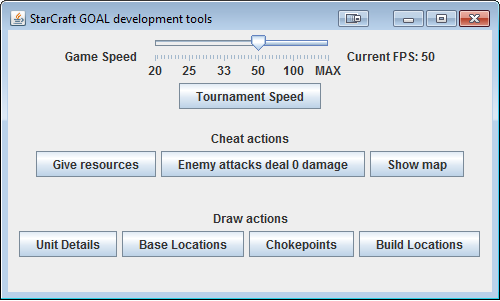
\includegraphics[width=1.0\textwidth]{images/developmentTool}
\caption{Example of the Development Tool}
\label{fig:StarCraft_picture}
\end{figure}

\subsection{Game Speed}
The Game Speed slider can be found at the top of the development tool window. This can be used to quickly change the speed of the game. The initial game speed is set to 50 fps (logical frames). The slowest speed is 20 fps and from there you can set it as fast as you want. Please note that the agent is supposed to play normally at 50 fps which is the default game speed for AI tournaments. When the speed is set to a 100 fps or higher, the agents can react slower than they would on the tournament gamespeed. Setting the game speed on 100 or higher should only be used for quick testing purposes.

\subsection{Cheat Actions}
The development tool offers 3 buttons which instantly enable StarCraft cheats. Note that these cheats should be used for testing purposes only. The first cheat is called: \textit{Give resources} which gives the player 10000 minerals and 10000 gas. The second cheat is called: \textit{Enemy attacks deal 0 damager} which makes the units of the player immune for damage. The last cheat is called: \textit{Show map} which makes the whole map visible for the player. Note that  all your agents will then also perceive everything on the map.

\subsection{Map Drawing}
The development tool can also be used to show map or unit details. There are 4 buttons which can be used. First there is the \textit{Unit Details} button which shows the health and \textit{ID} of every unit. There is also the \textit{Base Locations} button which shows all the starting locations of the map and also all the base locations on the map where players could be expanding to. There is also the \textit{Chokepoints} button which shows all the chokepoints (which are the narrow points where not many units can go through at the same time) on the map. Finally there is the \textit{Build Locations} button which shows all the non-obstructed and explored building locations of the map which the worker units perceive with the \textit{constructionSite} percept.